\chapter{General \RV}
The \rv used in this chapter takes a continuous range of possible values. There is a striking similarity between techniques used to manipulate discrete and continuous \rv.

\section{Continous \rv and PDFs}
A \rv $X$ is called continuous if there is a \textit{non-negative} function $f_X$ called the probability density function of $X$, or PDF, such that
\[\boxed { P(X\in B) = \int_B f_X(x) dx }\]
for every subset $B$ of real line. The probability that $X$ falls within the interval $[a,b]$ is
\[P(a \le X \le b) = \int_a^b f_X(x) dx\]
can be interpreted as the area under the graph of the PDF (see Fig. 3.1).

\begin{figure}[h]
    \center
    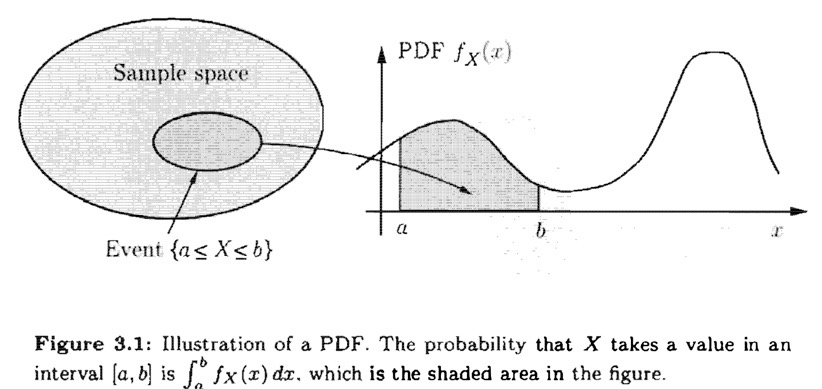
\includegraphics[width=.8\textwidth]{images/P_pdf.jpeg}
 \end{figure}

 For a single value $a$, we have $P(X=a)=\int_a^a f_X(x) dx = 0$. For this reason including or excluding the end points of an interval has no effect on its probability.

 \subsection{Interpretation of PDFs}
 Note that for small intervals $[x,x+\delta]$, we have
 \[P([x,x+\delta]) = \int_x^{x+\delta} f_X(t)dt \approx f_X(x) \cdot \delta\]

 We can view PDFs as the "probability mass per unit length" near $x$ (see Fig. 3.2). 

 Although PDFs are used to calculate the event probabilities, $f_X(x)$ is not the probability of any particular event. In particular, it is not restricted to be less than or equal to one.

 \begin{figure}[h]
    \center
    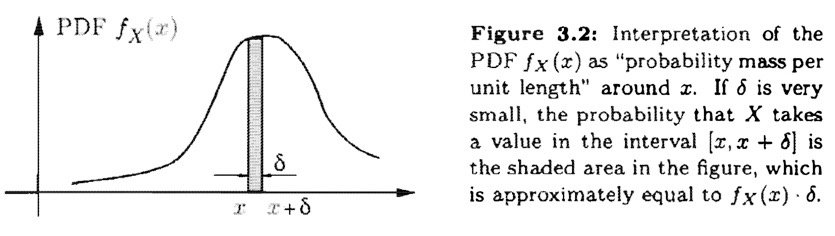
\includegraphics[width=.8\textwidth]{images/P_pdf_interpret.jpeg}
 \end{figure}

 \subsubsection{Example: PDF can take arbitrarily large values.}
 Consider  a \rv $X$ with PDF
 \[f_X(x) = \begin{cases}
     \frac{1}{2\sqrt{x}} & 0 < x \le 1 \\
     0 & \text{otherwise}
 \end{cases}\]

 This is still a valid PDF even when $f_X(x)$ becomes infinitely large as $x$ approaches zero because
 \[\int_{-\infty}^{+\infty}f_X(x) dx = \int_0^1 \frac{1}{2\sqrt{x}} dx = \sqrt{x}\Bigr|_0^1 = 1\] \qed

 \subsection{Properties of a PDF}
 \begin{enumerate}
     \item The function $f_X$ must be non-negative, i.e., $f_X(x) \ge 0$ for all $x$.
     \item For any subset $B$ of real line,
     \[P(X \in B) = \int_B f_X(x) dx\]
     \item The normalization property must hold
     \[\int_{-\infty}^{+\infty}f_X(x) dx=P(-\infty < X < +\infty) = 1\]
     This means that the area under the PDF must integrate to 1.
     \item If $\delta$ is very small, then $P([x,x+\delta]) \approx f_X(x) \cdot \delta$
 \end{enumerate}

 \subsection{Expectation}
 The expected value or mean of a continuous \rv $X$ is defined by
 \[ \boxed{\E [X] = \int_{-\infty}^{+\infty}xf_X(x) \; dx }\]

 This is similar to the discrete case except that 
 \begin{enumerate}
    \item PMF is replaced by the PDF.
    \item The summation is replaced by the integral.
 \end{enumerate}

 $\E[X]$ can be interpreted as the "center of gravity" of the PDF and also as the anticipated average value of $X$ over a large number of independent trails of the experiment. Its mathematical property is same as the discrete case --- after all the integral is just a limiting form of a sum.

 If $X$ is a continuous \rv with PDF $f_X(x)$ then $g(X)$ can be either a continuous or discrete \rv with the following properties
 \begin{itemize}
     \item Expected value is given by
     \[\E[g(X)]=\int_{-\infty}^{+\infty}g(x)f_X(x) \; dx\]
     \item The variance of $X$ is defined by
     \[\text{var}(X)=\E[(X-\E[X])^2]=\int_{-\infty}^{+\infty}(x-\E[x])^2 f_X(x) \; dx\]
     \item We have
     \[0 \le \text{var}(X)=\E[X^2]-\E[X]^2\]
     \item If $Y=aX+b$, where $a$ and $b$ are scalars, then
     \[\E[Y]=a\E[X]+b, \qquad \text{var}(Y)=a^2\text{var}(X)\]
 \end{itemize}

 \section{Cumulative Distribution Functions}
 CDFs provides a unified mathematical concept to deal with PMFs in discrete case and PDFs in continuous case. It helps to abstract the nature of the random variable.

 The CDF for a \rv is denoted by $F_X(x)$ and is the probability $P(X \le x)$. In particular, for every $x$ we have
 \[\boxed{
     F_X(x)=P(X \le x) = \begin{cases}
         \sum_{k \le x}p_X(k) & X \text{ is discrete} \\
         \int_{-\infty}^{x}f_X(t) \; dt & X \text{ is continuous}
     \end{cases}
 }\]
 
 Since $\{X\le x \}$ is always an event and has a well defined probability and therefore any unambiguous specification of the probabilities of all events of the same form (through PMF, PDF or CDF) will be referred as the probability law of the \rv $X$.

 \subsection{Properties of CDF}
 The CDF $F_X(x)$ of a \rv $X$ satisfies
 \begin{enumerate}
     \item $F_X(x)$ is monotonically non-decreasing.
     \item The limiting value of CDF are 
     \[\lim_{x \to -\infty}F_X(x) = 0, \qquad \lim_{x \to +\infty}F_X(x) = 1\]
     \item If $X$ is discrete then PMF and CDF can be obtained from each other by
     \[F_X(x)=\sum_{i=-\infty}^{k} p_X(i)\]
     \[p_X(k)=P(X\le k) - P(X\le k-1)=F_X(k)-F_X(k-1)\]
     \item If $X$ is continuous, the PDF and CDF can be obtained from each other by
     \[F_X(x)=\int_{-\infty}^{x}f_X(t) dt, \qquad f_X(x)=\frac{dF_X(x)}{dx}\]
     The second equality holds on points where PDF is continuous.
 \end{enumerate}

 \subsubsection{Example: Maxmium of Several \RV}
You are allowed to take a test 3 times and the final score will be the maximum out the three. Score ranges from 1 to 10 with equal probability independently of other tests. Calculate PMF of the final score.

This problem can be easier to attempt by first calculating CDF and then differencing to calculate the PMF. We have
\begin{align*}
    F_X(k) &= P(X \le k) = P(X_1 \le k, X_2 \le k, X_3 \le k) \\
           &= P(X_1 \le k)P(X_2 \le k)P(X_3 \le k) \\
           &= \left(\frac{k}{10}\right)^3 \\
\end{align*}
Thus the PMF is given by
\[p_X(k)=F_X(k)-F_X(k-1)=\left(\frac{k}{10}\right)^3 - \left(\frac{k-1}{10}\right)^3, \qquad k=1,2,\ldots, 10\]
\qed

\section{Normal Random Variable}
A continuous \rv $X$ is said to be normal or Gaussian if it has a PDF of the form
\[\boxed{ f_X(x) = \frac{1}{\sqrt{2\pi}\sigma}\exp\left({\frac{-(x-\mu)^2}{2\sigma^2}}\right) }\]

Where $\mu$ and $\sigma > 0$ are two scalar parameters  characterizing the PDF by denoting mean and standard deviation respectively. Normalization property can be verified.

\subsection{Linear transformation of a Normal \rv}
If $X$ is a normal \rv with mean $\mu$ and variance $\sigma^2$ and if $a \neq 0$, $b$ are scalars, then the \rv $Y=aX+b$ is also a normal \rv with
\begin{align*}
    \E[Y]          &= a\mu + b \\ 
    \text{var} (Y) &= a^2\sigma ^2
\end{align*}

\subsection{Standard Normal \RV}
The normal \rv $X$ with zero mean and unit variance is said to be a standard normal. Its CDF is denoted by $\Phi$
\[\Phi (x)=P(X \le x)=P(X<x)=\int_{-\infty}^{x}e^{t^2/2} \; dt\]

The values of this are recorded in a table and is useful in calculating probabilities involving normal \rv.

The tables only provides values of $\Phi (x)$ for $x\ge 0$, because the omitted values can be found by the symmetry of the PDF. For example, if $X$ is a standard normal then
\[\Phi(-0.5)=\Phi(X\le -0.5)=\Phi(X\ge 0.5)=1-\Phi(0.5)\]
More generally we have $\Phi(-x)=1-\Phi(x)$, $\forall x$.

Let $X$ be a normal \rv with mean $\mu$ and variance $\sigma^2$. We standardize $X$ be defining a new \rv $Y$. Since $Y$ is a linear transformation of $X$ it is normal. Further
\[
    Y=\frac{X-\mu}{\sigma}, \qquad \E[Y] = \frac{\E[X]-\mu}{\sigma}=0, \qquad \text{var}(Y)=\frac{\text{var}(X)}{\sigma^2}=1
\]
Thus $Y$ is a standard normal \rv and this allows us to calculate CDF for a normal \rv by
\begin{enumerate}
    \item "Standardize" $X$ and obtain $Y$ by the above transformation.
    \item Read the CDF from the standard normal table
    \[P(X\le x)=P\left(\frac{X-\mu}{\sigma} \le \frac{x-\mu}{\sigma}\right)=\Phi\left(\frac{x-\mu}{\sigma}\right)\]
\end{enumerate}

\section{Joint PDF of Multiple \RV}
The two random variables associated with the same experiment are jointly continuous and can be described in terms of joint PDF $f_{X,Y}$ which is a nonnegative function that satisfies
\[ \boxed { P((X,Y)\in B) = \iint_{(x,y)\in B}f_{X,Y}(x,y) \; dx \, dy }\]

for every subset $B$ of the 2D plane.
\subsection{Properties of Joint PDF}
\begin{enumerate}
    \item Letting $B$ to be the entire 2D plane, we get the \textbf{normalization} property
    \[\int_{-\infty}^{+\infty}\int_{-\infty}^{+\infty}f_{X,Y}(x,y) \; dx \, dy = 1\]
    \item Letting $B$ to be a small rectangle of side length $\delta$
    \[P(a\le X \le a+\delta, c \le Y \le c+\delta) = \int_{c}^{c+\delta}\int_{a}^{a+\delta}f_{X,Y}(x,y) \; dx \, dy \approx f_{X,Y}(a,c) \cdot \delta^2\]
    Thus $f_{X,Y}(a,c)$ is the \textbf{probability per unit area} in the vicinity of $(a,c)$.
    \item \textbf{Marginal PDFs} are given by
    \[f_X(x)=\int_{-\infty}^{+\infty}f_{X,Y}(x,y) \, dy, \qquad f_Y(y)=\int_{-\infty}^{+\infty}f_{X,Y}(x,y) \, dx\]
    Thus for any subset $A$ of the real line, consider the event $\{X\in A\}$
    \[P(X\in A)=P(X\in A,-\infty \le Y \le +\infty) = \int_A \int_{-\infty}^{+\infty} f_{X,Y}(x,y) \, dy \, dx\]
\end{enumerate}

\begin{example}[Buffon Needle Problem]
A surface is ruled with parallel lines separated by $d$ and a needle of length $l$ is thrown at random. Find the probability that the needle intersect one of the lines.


We assume $d > l$ so that the needle cannot intersect both of the lines simultaneously. 

\begin{figure}[h]
    \center
    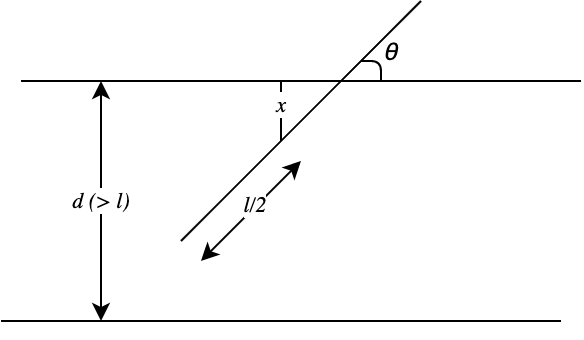
\includegraphics[width=.4\textwidth]{images/P_buffon_needle.png}
 \end{figure}
 
The distance of the midpoint from the closest line is $x$. The needle forms an acute angle $\theta$ with the horizontal line.  The needle length corresponding to the intersection is $x/\sin \theta$. The needle will intersect the line if this distance is less than $l/2$.

We model this using random variables $(X,\Theta)$. It can be seen since the throw is random the vertical orientation is uniformly distributed along with the orientation of the needle. This means that both of the \rv are independent. Since all throws are equally likely the joint PDF will be uniformly distributed over all $x \in [0, d/2]$ and $\theta \in [0,\pi/2]$. Thus this gives us the following joint PDF
\[f_{X,\Theta}=\begin{cases} 
    4/(\pi d) & x \in [0, d/2], \theta \in [0, \pi/2] \\
    0 & \text{otherwise}
\end{cases}\]

The needle can only intersect the line when $X \le (l/2)\sin \Theta$. So the probability of intersection is 
\[P(X \le (l/2)\sin \Theta) = \int_{0}^{\pi/2}\int_{0}^{(l/2)\sin \theta} \frac{4}{\pi d} \, dx \, d\theta = \frac{2l}{\pi d}\] \qed
\end{example}

\subsection{Joint CDFs}
If $X, Y$ are two \rv associated with the same experiment then we define the Joint CDF as
\[\boxed {F_{X,Y}(x,y) = P(X\le x, Y\le y)}\]

The advantage of working with Joint CDFs is that it allows us to deal with both --- discrete and continuous random variable in one shot.

The PDFs can be recovered from CDF by differentiating
\[\boxed{f_{X,Y}(x,y)=\frac{\partial^2{F_{X,Y}}}{\partial x \, \partial y}(x,y)}\]

\subsection{Expectation}
For two jointly continuous \rv $X, Y$ and $Z=g(X,Y)$ is also a \rv for some function $g$. The expected value is given by
\[\E[g(X,Y)]=\int_{-\infty}^{+\infty}\int_{-\infty}^{+\infty}g(x,y)f_{X,Y}(x,y) \, dx \, dy\]

For any scalars $a, b, c$ we have,
\[\E[aX+bY+c]=a\E[X]+b\E[Y]+c\]

\section{Conditioning}
The formulas for conditional probabilities are similar to that of the discrete case except the subtlety that arises because of the event $\{Y=y\}$ which has zero probability.

\subsection{Conditioning a \RV on an event}
The conditional PDF of a continuous \rv given an event $A$ with $P(A)>0$ is defined as a nonnegative function $f_{X|A}(x)$ that satisfies
\[\boxed{P(X \in B| A) = \int_{B}f_{X|A}(x) dx}\]
for any subset $B$ of the real line. For setting $B$ to be entire real line, we obtain the normalization property
\[\int_{-\infty}^{+\infty}f_{X|A}(x) \, dx =1\]
Thus $f_{X|A}$ is a legitimate PDF.

As a special case
\[f_{X|X\in A}(x) = \begin{cases}
   \dfrac{f_X(x)}{P(X\in A)}, & x \in A \\
    0, & \text{otherwise}
\end{cases}\]
Similarly there is a notion of joint conditional PDF of two jointly associated \rv $X,Y$ with joint PDF $F_{X,Y}(x,y)$. For a conditioning event $C=\{(X,Y)\in A\}$, we have
\[f_{X,Y|C}(x,y)=\begin{cases}
    \dfrac{f_{X,Y}(x, y)}{P(C)}, & x \in A \\
     0, & \text{otherwise}
 \end{cases}\]
The conditioning PDF of $X$ can be obtained from the formula
\[f_{X|C}(x) = \int_{-\infty}^{+\infty} f_{X,Y|C}(x,y) dy\]

Finally, there is a version of total probability theorem which involves conditional PDFs: if events $A_1, \ldots, A_n$ form a partition of the sample space then
\[\boxed {f_X(x) = \sum_{i=1}^{n} P(A_i)f_{X|A_i}(x)}\]

\subsection{Conditioning one \RV on Another}
Let $X, Y$ be continuous \rv with joint PDF $f_{X,Y}(x,y)$. For any $y$ with $f_Y(y)>0$, the conditional PDF of $X$ given that $Y=y$, is defined by 
\[\boxed{f_{X|Y}(x|y) = \frac{f_{X,Y}(x,y)}{f_Y(y)}}\]

It is best to think $y$ as a fixed number so that the conditional PDF $f_{X|Y}(x|y)$ is a function of a single variable $x$ with same shape as the $f_{X,Y}(x,y)$ because the denominator doesn't depend on $x$.

Since the following normalization property holds, $f_{X|Y}(x,y)$ is a legitimate PDF for a fixed $y$.
\[\int_{-\infty}^{+\infty}f_{X|Y}(x|y)\,dx=1\]

\subsubsection{Interpretation of conditional PDFs}
Consider two small positive numbers $\delta_1, \delta_2$ and the conditioning event $B={Y\in [y, y+\delta_2]}$, we have
\begin{align*}
    P(X \in [x, x+\delta_1]|Y \in [y, y+\delta_2]) & =\frac{P(X \in [x, x+\delta_1],Y \in [y, y+\delta_2])}{P(Y \in [y, y+\delta_2])} \\
    & \approx \frac{f_{X,Y}(x,y)\delta_1\delta_2}{f_Y(y)\delta_2} \\
    &= f_{X|Y}(x|y)\delta_1
\end{align*}

In other words, $f_{X|Y}(x|y)\delta_1$ provides us with the probability $X \in [x,x+\delta_1]$ given that $Y\in [y, y+\delta_2]$. Since the probability does not depend on $\delta_2$ we can consider the limiting case where $\delta_2 \to 0$ and write
\[P(X\in[x,x+\delta_1]|Y=y) \approx f_{X|Y}(x|y)\delta_1\]
or more generally
\[P(X \in A|Y=y) = \int_{A}f_{X|Y}(x|y) \, dx\]

Note that the event $\{Y=y\}$ is a zero probability event and in discrete case it was left undefined unlike the current formula which is natural.

As in the discrete case, the conditional probability $f_{X|Y}$ is used along with $f_Y(y)$ to calculate the joint PDFs. This approach can be used for modelling the joint probability where the event of $Y$ is specified and then the conditional probability $f_{X|Y}(x|y)$ of $X$ are specified.

\begin{align*}
    f_{X,Y}(x,y) &= f_Y(y)f_{X|Y}(x|y) \\
    f_X(x) &= \int_{-\infty}^{+\infty}f_Y(y)f_{X|Y}(x|y) \, dy
\end{align*}

The above results can be easily extended to more than one variable.

\subsection{Conditional Expectation}
Let $X, Y$ be jointly continuous \rv and let $A$ be an event with $P(A)>0$
\begin{enumerate}
    \item The conditional expectation of $X$ given the event $A$ is defined by 
    \[\E[X|A]=\int_{-\infty}^{+\infty}xf_{X|A}(x) \, dx, \qquad
    \E[X|Y=y] = \int_{-\infty}^{+\infty}xf_{X|Y}(x|y) \, dx\] 
    \item \textbf{The expected value rule}: For a function $g(X)$ we have
    \[\E[g(X)|A] = \int_{-\infty}^{+\infty} g(X) f_{X|A}(x)dx, \qquad 
    \E[g(X)|Y=y] = \int_{-\infty}^{+\infty}g(x)f_{X|Y}(x|y) \, dx\]
    \item \textbf{Total expectation theorem:} Let $A_1,\ldots,A_n$ be disjoint events that form a partition of the sample space and assume that $P(A_i)>0, \; \forall i$. Then,
    \[\E[X] = \sum_{i=1}^{n} P(A_i) \E[X|A_i], \qquad \E[X] = \int_{-\infty}^{+\infty}\E[X|Y=y] f_Y(y) \, dy\]
    \item There are natural analogs for the case of functions of several \rv 
    \[\E[g(X,Y)|Y=y] = \int g(x,y)f_{X|Y}(x|y) dx, \qquad E[g(X,Y)] = \int \E[g(X,Y)|Y=y] f_Y(y) \, dy\]
\end{enumerate}

\section{Independence}
In full analogy to the discrete case we say that the two \rv $X, Y$ are independent if
\[\boxed {f_{X,Y}(x,y) = f_X(x)f_Y(y) \qquad \forall x,y}\]
which is same as
\[f_{X|Y}(x|y) = f_X(x), \quad \forall x,y; \; f_Y(y)>0\]
Some other properties are
\begin{enumerate}
    \item In particular, independence implies
    \[F_{X,Y}(x,y)=P(X\le x, Y\le y)=P(X\le x)P(Y\le y)=F_X(x)F_Y(y)\]
    \item The above can be used to provide a general definition for the independence
    \[F_{X,Y}(x,y) = F_X(x)F_Y(y) \qquad \forall x,y\]
    Even if $X$ is discrete and $Y$ is continuous.
    \item If $X, Y$ are independent then
    \[\E[g(X)h(Y)] = \E[g(X)]\E[h(Y)]\]
    \item The variance of sum of independent random variables is equal to the sum of their variances.
    \begin{center}
        var$(X+Y)$ = var$(X)$ + var$(Y)$
    \end{center}
\end{enumerate}

\section{Continuous Bayes' Rule}
The setting is similar to the discrete case and the only difference is the continuous \rv here. The cases discussed below are based on whether quantity observed or inferred is continuous.

\begin{figure}[h]
    \center
    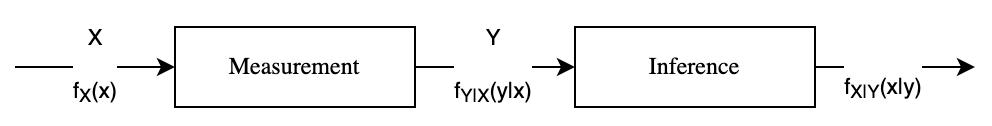
\includegraphics[width=.8\textwidth]{images/P_bayes rule.png}
 \end{figure}

Let the unobserved phenomenon is denoted by a \rv $X$ with known PDF $f_X$. We obtain a measurement $Y$ according to a conditional PDF $f_{Y|X}$. Given the observed value $y$ of $Y$, the inference problem is to evaluate the conditional PDF $f_{X|Y}$.

Note that whatever information is provided by the event $\{Y=y\}$ is captured by the conditional PDF $f_{X|Y}$. It suffices us to calculate this PDF.
\begin{align*}
    f_{X|Y}(x|y) &= \dfrac{f_{X,Y}(x, y)}{f_Y(y)} \\
                &= \dfrac{f_X(x)f_{Y|X}(y|x)}{\int_{-\infty}^{+\infty}f_X(t)f_{Y|X}(y|t) \, dt}
\end{align*}

\subsection{Inference about a discrete \rv}
Let the unobserved phenomenon is described in terms of an event $A$ whose occurrence is unknown. Let $P(A)$ denotes its probability. Let $Y$ be a continuous \rv and assume that $f_{Y|A}$ and $f_{Y|A^c}$ are known. We are interested in $P(A|Y=y)$ of the event $A$, given the that $Y$ takes $y$.

Instead of working with the event zero probability event $\{Y=y\}$, let us work with $\{y \le Y \le y+\delta\}$ where $\delta$ is a small positive number and then take the limit tending to zero. We have using Bayes' rule and assuming $f_Y(y)>0$
\begin{align*}
    P(A|Y=y) & \approx P(A|y \le Y \le y+\delta) \\
             &= \frac{P(A)P(y \le Y \le y+\delta|A)}{P(y \le Y \le y+\delta)} \\
             & \approx \frac{P(A)f_{Y|A}(y)\delta}{f_Y(y)\delta} \\
             &= \frac{P(A)f_{Y|A}(y)}{f_Y(y)}\\
             &= \frac{P(A)f_{Y|A}(y)}{P(A)f_{Y|A}(y)+P(A^c)f_{Y|A^c}(y)}
\end{align*}

The last equality follows because of the total probability theorem.

\subsection{Inference Based on Discrete Observations}
Note that
\begin{align*}
    f_{Y|A}(y) &= \frac{f_Y(y)P(A|Y=y)}{P(A)} \\
               &= \frac{f_Y(y)P(A|Y=y)}{\int_{-\infty}^{+\infty}f_Y(t)P(A|Y=t) \, dt}
\end{align*}

This formula can be used to make an inference about a \rv $Y$ when event $A$ is observed. 